\section{Results and discussion} \label{Results-and-discussion}

\subsection{Thorium feed mechanism}

The first mechanism adopts continuous feed flow of external thorium and 
$^{233}$U from \texttt{Pa-decay tank}. Hereinafter the first mechanism will be 
mentioned as the thorium feed mechanism. The molar fraction of the heavy metal 
in the initial fuel was kept constant and equal to 12.5 mole\% for all cases. 
Besides, the initial fissile material fraction was increased for the five fuel 
salt compositions until the \gls{SD-TMSR} reactor was sufficiently critical at 
the Beginning Of Life (BOL). 
Figure~\ref{fig:keff1} illustrates the change of the effective multiplication with \gls{EFPY} for the thorium feed mechanism. As shown in Figure~\ref{fig:keff1}, the effective multiplication factor ($k_{eff}$) decreases sharply during the first 25 years of reactor operation for the first four cases. $k_{eff}$ decreases as a result of depletion of the initial fissile materials and generation of the neutron poisons (FPs). Thus, the reactor becomes subcritical within a relatively short time ($\approx$ $4$ $years$ in the \gls{TRU} case and $\approx$ $12$ $years$ in the Pu reactor-grade case). The amount of $^{233}$U generated in the \gls{SD-TMSR} is not enough to conserve the reactor criticality and overcome the neutron absorption in the initial fertile isotopes. Nevertheless, the continuous feed flow of thorium and $^{233}$U helps to operate the \gls{SD-TMSR} for a long period of time (the U-233 case). Additionally, the initial molar fraction in the LEU and Pu reactor-grade cases was increased more (see Figure~\ref{fig:keff1}) to counteract the absorption of neutrons in the non-fissile heavy metals added with the initial fuel salt. But $k_{eff}$ still decreases below 1.0, as a result of increasing the non-fissile heavy metals in the initial fuel \cite{betzler2016modeling}.

\begin{figure}
	\centering
	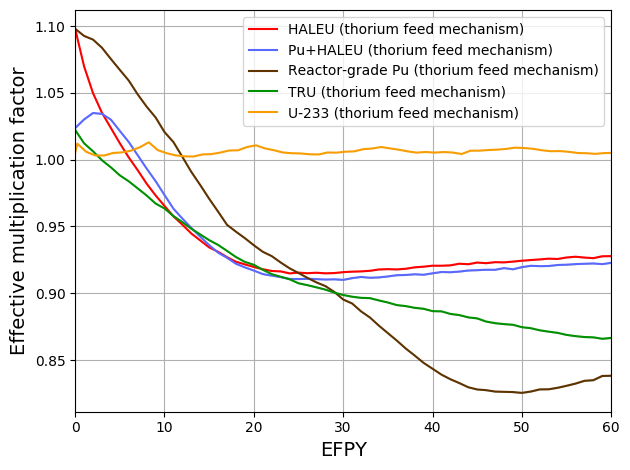
\includegraphics[width=\textwidth]{keff1.png}
	\caption{The change of the effective multiplication factor during 60 \gls{EFPY} of reactor operation for thorium feed mechanism (confidence interval $\pm\sigma$ is shaded).} 
	\label{fig:keff1}
\end{figure}

\subsection{Non-thorium feed mechanism}

The second mechanism allows continuous feed flow of $^{233}$U from \texttt{Pa-decay tank} and Heavy Metal except for Th. Hereinafter the second mechanism will be mentioned as the non-thorium feed mechanism. Figure~\ref{fig:keff2} shows the change of the effective multiplication during 60 \gls{EFPY} of reactor operation for the non-thorium feed mechanism.
As shown in Figure~\ref{fig:keff2}, the SD-TMS reactor was sufficiently critical at the Beginning Of Life (BOL). Both Pu reactor-grade and TRU case show promising results relative to the other two cases (i.e. LEU and Pu+LEU). For the Pu reactor-grade fuel salt, the amount of $^{233}$U generated in the \gls{SD-TMSR} in addition to the external feed flow of Pu are sufficient to maintain the reactor criticality and overcome the neutron absorption in the initial non-fissile isotopes. This may be attributed to the fact that the spectrum in the Pu reactor-grade initial core is hardened that is more thorium is being converted to $^{233}$U. For the \gls{TRU} fuel salt, the amount of $^{233}$U and the external feed flow of TRU is barely enough to operate the reactor for a long period of time ($\approx$ $40$ $years$) without any external feed of $^{233}$U. Nevertheless, $k_{eff}$ decreases with the burnup because the Minor Actinides\footnote{In the present work, the Minor Actinides (MA) include Np, Am and Cm.} (MA) accumulating in the core as a result of continuous TRU feed. As shown in Figure~\ref{fig:keff2}, the LEU and Pu+LEU fuel are less attractive for non-thorium feed mechanism. The continuous LEU feed increases the amount of fertile $^{238}$U and consequently, reduces the feasibility of such fissile materials. The continuous feed of $^{233}$U without $^{232}$Th will lead to supercritical reactor, thus the $^{233}$U case is excluded from non-thorium feed mechanism.\\
According to the $k_{eff}$ results, Pu reactor-grade and TRU fissile materials are selected and discussed in the following. 
\begin{figure}
	\centering
	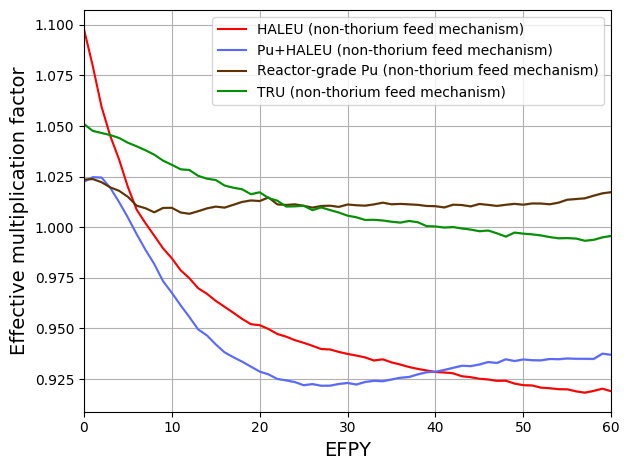
\includegraphics[width=\textwidth]{keff2.png}
	\caption{The change of the effective multiplication factor during 60 \gls{EFPY} of reactor operation for non-thorium feed mechanism (confidence interval $\pm\sigma$ is shaded).} 
	\label{fig:keff2}
\end{figure}

\subsection{Pu reactor-grade, TRU, and $^{233}$U initial fuel}

In this section, the simulation of the SD-TMSR with Pu reactor-grade and TRU fissile materials is discussed. Besides, the $^{233}$U case is listed for comparison.\\
Figure~\ref{fig:refillCCC} demonstrates the dynamics of heavy metal refill rate during 60 \gls{EFPY} of SD-TMSR operation. The heavy metal refill rate was adjusted to maintain; the reactor criticality and total fuel mass almost constant\footnote{The variation of the total fuel mass is less than $0.1\%$} during the reactor operation. In $^{233}$U case, the mean values of $^{233}$U and $^{232}$Th refill rate are $1.77$ and $2.21$ $kg/d$, respectively. As well, in the Pu reactor-grade case, the mean values of $^{233}$U and Pu refill rate are $0.75$ and $2.75$ $kg/d$, respectively. In the TRU case, the mean values of $^{233}$U and TRU refill rate are $0.90$ and $2.0$ $kg/d$, respectively.

\begin{figure}
	\centering
	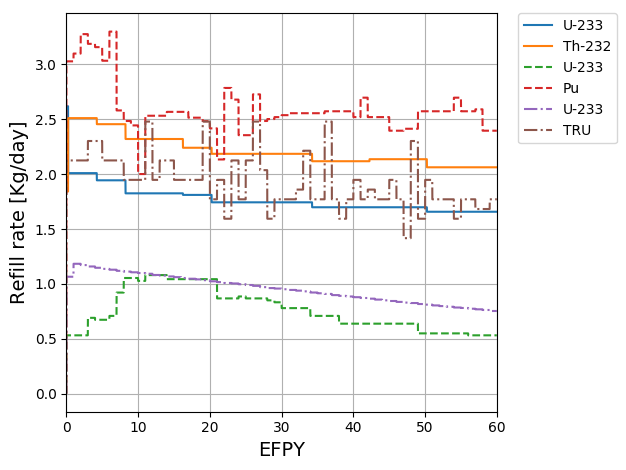
\includegraphics[width=\textwidth]{refillCCC.png}
	\caption{Dynamics of heavy metal refill rate during 60 \gls{EFPY} of reactor operation. Solid lines for $^{233}$U case, dashed lines for Pu reactor-grade case, and dotted lines for TRU case.}
	\label{fig:refillCCC}
\end{figure}

Figure~\ref{fig:inventoryCCCC} and ~\ref{fig:inventoryPu_TRUCCC} describe the evolution of important isotopes for $^{233}$U, Pu and TRU cases respectively.
From Figure~\ref{fig:inventoryCCCC}, the mass of Pa in the fuel salt is almost constant and reaches $17.8$  $kg$ at the end of the operation time. In addition, the mass of Minor Actinides (MA) increases with time; however, by applying online reprocessing, its value remains relatively low. As well, the total mass of Pu increases with burnup. The level of Pu in the fuel correlates with the mass of the MA, and Pu. MA need more time to reach equilibrium. The total mass of U increases with burnup and reaches equilibrium after $\approx$ $27$ $years$. As shown in Figure~\ref{fig:inventoryCCCC}, refueling the core with Th helps maintain an almost constant inventory throughout the full operation time.\\
The Pa extraction time was adjusted to be 30 seconds for Pu and TRU cases to avoid poisoning the core. Therefore, Figure~\ref{fig:inventoryPu_TRUCCC} shows that the mass of Pa in the fuel for Pu and TRU cases is relatively low when compared to the $^{233}$U case.
Major isotopes for the three cases reaches the equilibrium state after $\approx$ $30$ $years$ (see Figure~\ref{fig:inventoryCCCC} and ~\ref{fig:inventoryPu_TRUCCC}).

\begin{figure}
	\centering
	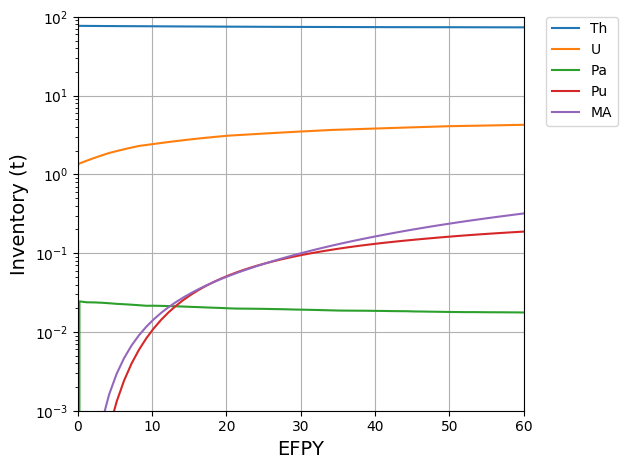
\includegraphics[width=\textwidth]{inventoryCCCC.png}
	\caption{Evolution of the important nuclides inventories for $^{233}$U case (MA involves Np, Am, Cm).}
	\label{fig:inventoryCCCC}
\end{figure}

\begin{figure}
	\centering
	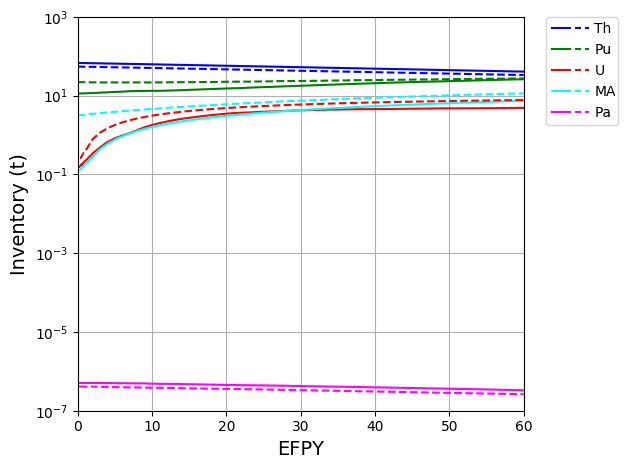
\includegraphics[width=\textwidth]{inventoryPu_TRUCCC.png}
	\caption{Evolution of the important nuclides inventories for Pu reactor-grade case (solid lines) and for TRU case (dashed lines).}
	\label{fig:inventoryPu_TRUCCC}
\end{figure}


Figure~\ref{fig:Th232CC} illustrates the variation of thorium mass in the fuel salt for $^{233}$U, Pu reactor-grade and TRU cases, respectively. In $^{233}$U case, we apply the thorium feed mechanism, thus thorium mass decreases by only $3.2$ $\%$ at the end of operation time (60 years). In contrast, thorium mass decreases significantly in Pu and TRU cases according to the non-thorium feed mechanism. Thorium mass decreases by $39.2$ $\%$ and $37.96$ $\%$ in Pu reactor-grade and TRU cases, respectively. The more decreasing in thorium mass, the more effective utilization of thorium fuel cycle. Consequently, the Pu reactor-grade initial fuel may help to utilize thorium fuel cycle more effective.

\begin{figure}
	\centering
	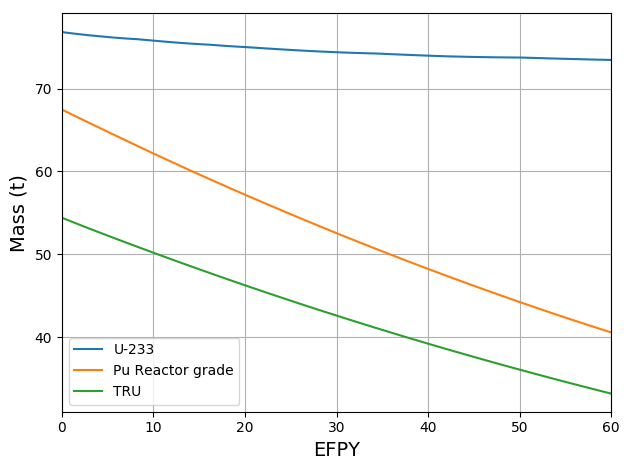
\includegraphics[width=\textwidth]{Th232CC.png}
	\caption{The variation of thorium mass in the fuel salt for $^{233}$U, Pu reactor-grade and TRU cases, respectively.}
	\label{fig:Th232CC}
\end{figure}

Figure~\ref{fig:U233CC} demonstrates the mass of $^{233}$U in the fuel salt for $^{233}$U, Pu reactor-grade and TRU cases, respectively. One can see that the mass of the $^{233}$U reaches the equilibrium state after $\approx$ $30$ $years$. Meanwhile, the amount of $^{233}$U is sufficient to maintain criticality in the three cases.

\begin{figure}
	\centering
	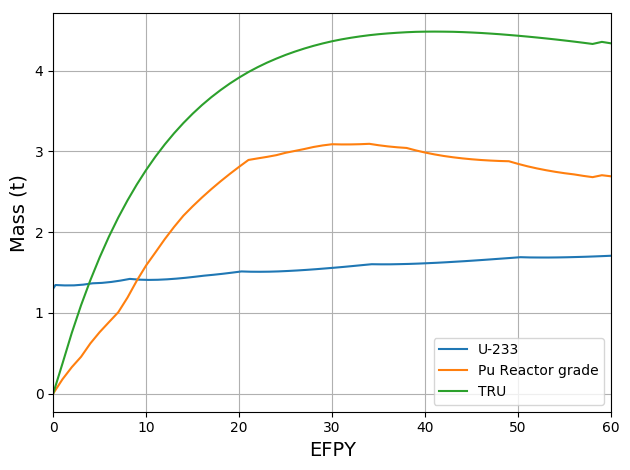
\includegraphics[width=\textwidth]{U233CC.png}
	\caption{Mass of $^{233}$U in the fuel salt for $^{233}$U, Pu reactor-grade and TRU case, respectively.}
	\label{fig:U233CC}
\end{figure}

In the non-thorium feed mechanism, the SD-TMSR is continuously refueled for criticality, which increases the Pu proportion in the molten salt. According to the literature, the limit of Pu solubility in the FLiBe salt is $\approx$ $4.0$ $\%$ \cite{ignatiev2012progress,sood1975plutonium}. Figure~\ref{fig:PusolubilityCC} represents the Pu proportion in the fuel salt (mole\%). In $^{233}$U and Pu reactor-grade cases, the Pu proportion increases slightly but still below its solubility limit. On the other hand, the Pu proportion in the molten salt loaded by TRU increases with operation time and reaches the Pu solubility limit after $\approx$ $40$ $years$. This issue may be solved by increasing the reactor operation temperature and or reducing the HM initial inventory \cite{zou2018transition}.

\begin{figure}
	\centering
	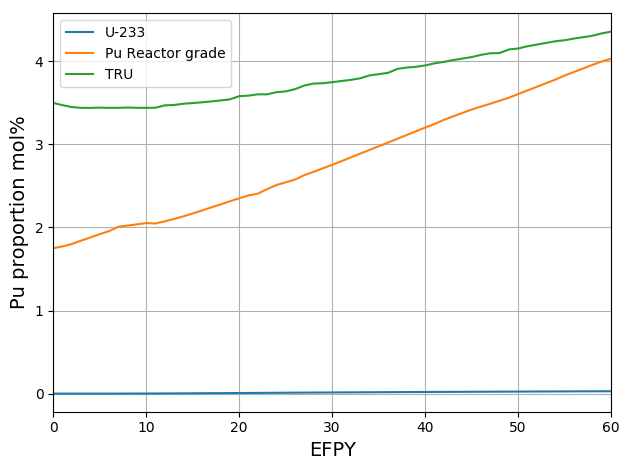
\includegraphics[width=\textwidth]{PusolubilityCC.png}
	\caption{The Pu proportion in the fuel salt (mole\%).}
	\label{fig:PusolubilityCC}
\end{figure}

Figure~\ref{fig:NetCC} demonstrates the net production of $^{233}$U as a 
function of burnup. In TRU case, the net production of $^{233}$U is almost 
zero, nevertheless, the reactor becomes subcritical after $40$ $years$ of 
operation. In $^{233}$U and Pu reactor-grade cases, the net production of 
$^{233}$U increases with burnup and reaches about $1.77$ $t$ and $10$ $t$, 
respectively at the end of operation lifetime. It worth noting that thorium 
feed mechanism is applied in $^{233}$U case, while, non-thorium feed mechanism 
is adopted in Pu reactor-grade cases.
As shown in Figure~\ref{fig:NetCC}, after 26 years the net production of $^{233}$U reaches $1.3$ $t$; this is sufficient to start-up another \gls{SD-TMSR}. Similarly, one can see that the same amount of $^{233}$U (i.e. $1.3$ $t$) can be achieved after $\approx$ $4.5$ $years$ if we applied the non-thorium feed mechanism on the SD-TMSR that initially loaded by Pu reactor-grade alternative to $^{233}$U. In addition, Figure~\ref{fig:NetCC} also shows that the net production of $^{233}$U during the first 455 days is negative, thus about $175.28$ $kg$ of $^{233}$U must be added during this period. In conclusion, the thorium fuel cycle transition can be achieved by selecting the proper feed mechanism and initial fissile material. 

\begin{figure}
	\centering
	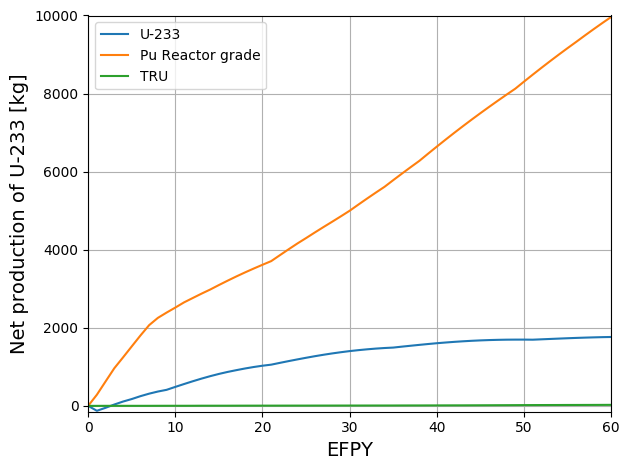
\includegraphics[width=\textwidth]{NetCC.png}
	\caption{Net production of $^{233}$U during burn-up period (60 \gls{EFPY}).}
	\label{fig:NetCC}
\end{figure}

\subsection{Neutron spectrum}

Figure~\ref{fig:spectrumFLUX110vC} represents the neutron flux per unit 
lethargy for full-core SD-TMSR model in the energy range from 10$^{-8}$ to 10 
MeV for the $^{233}$U, Pu reactor-grade, and TRU started case. In $^{233}$U 
case, at the EOL, the neutron spectrum is harder than at BOL due to the 
accumulation of the Pu and other strong thermal neutron absorbers in the fuel 
salt. For Pu reactor-grade and TRU cases, during the reactor operation, the 
fissile Pu is depleted and the $^{233}$U becomes the major fissile isotope 
(see Figure~\ref{fig:U233CC}), the neutron spectrum softens and becomes 
similar to a thermal spectrum of the TMSR.
 
\begin{figure}
 	\centering
 	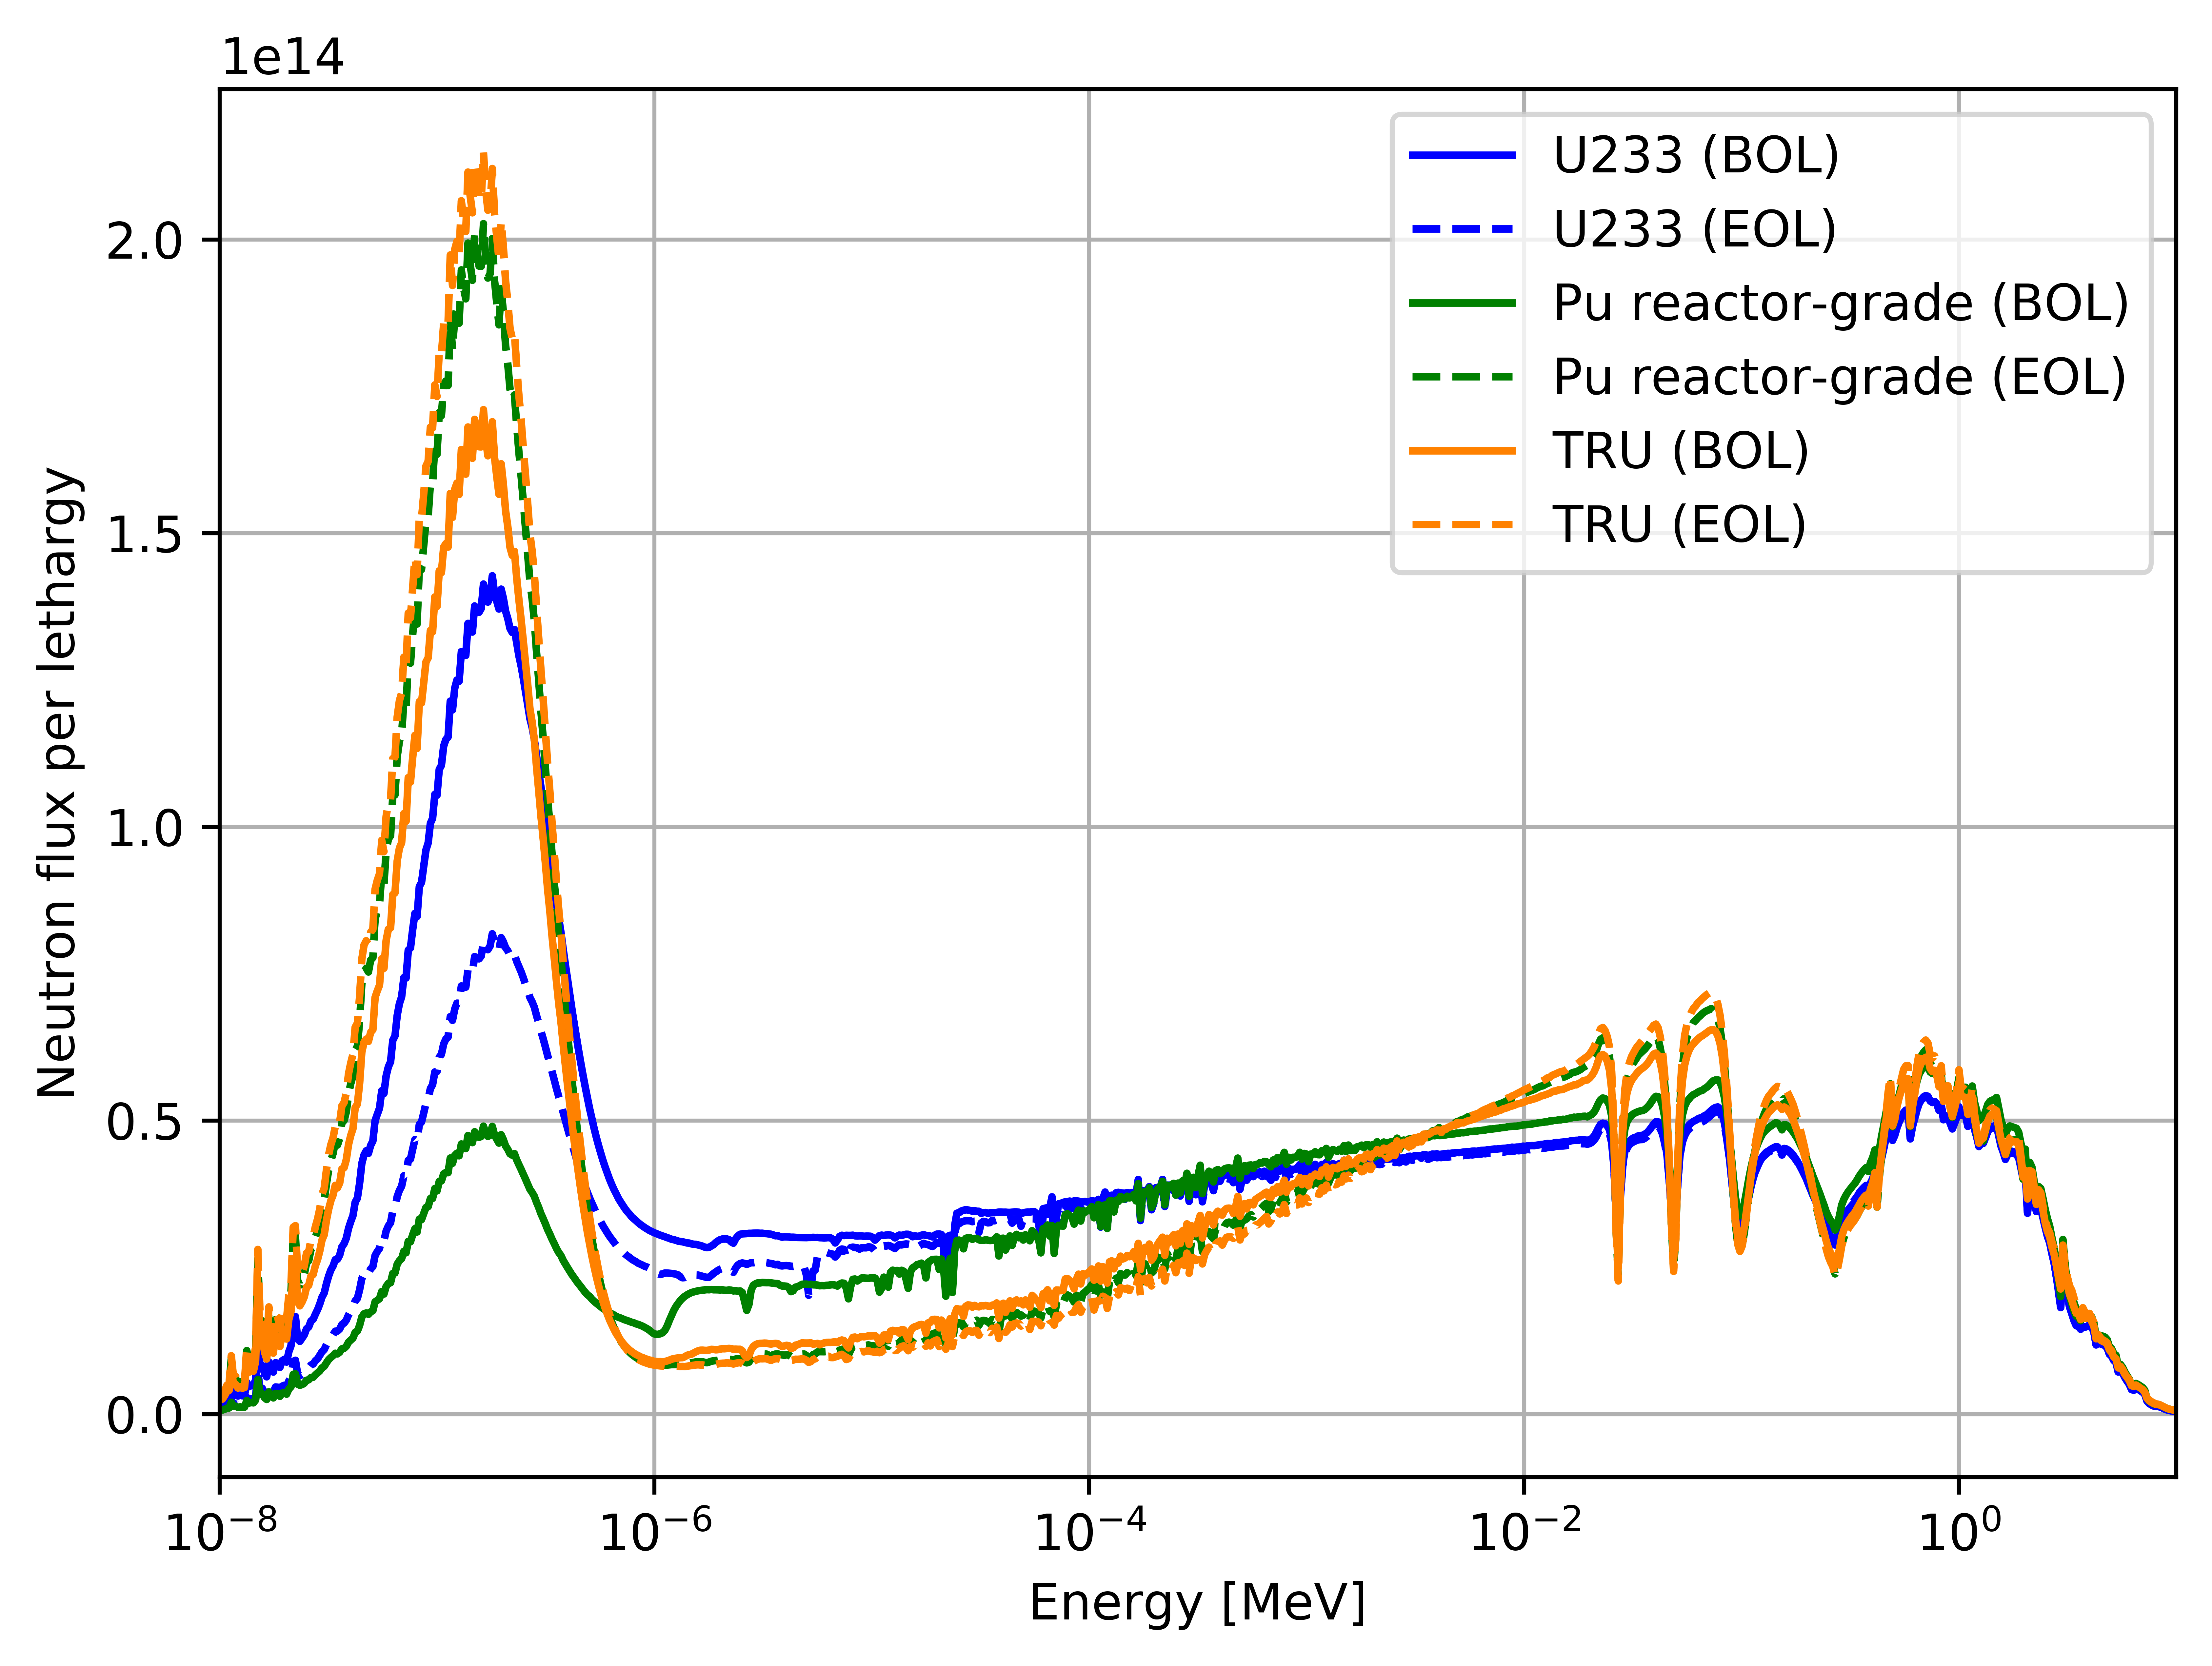
\includegraphics[width=\textwidth]{spectrumFLUX110vC.png}
 	\caption{The neutron flux energy spectrum at BOL (solid lines) and EOL (dashed lines) for $^{233}$U, Pu reactor-grade, and TRU case.}
 	\label{fig:spectrumFLUX110vC}
\end{figure}

The comparison between the two feed mechanisms with different types of initial fuel is listed in Table~\ref{tab:table7}. 
	
\begin{table} % [!ht]
	\centering
	\caption{Comparison between the two feed mechanisms for the five different types of initial fuel.}
	\vspace{0.1in}
	\begin{tabularx}{\textwidth}{l s s s s s }  %{\textwidth}
		\hline
		\backslashbox{Feed\\ mechanism}{Initial\\ fuel}& \gls{LEU} (19.79\%) & Pu mixed with enriched U (19.79 wt-\%) & Pu reactor-grade & \gls{TRU}& $^{233}$U \\
		\hline
		Thorium feed mechanism&Not work&Not work&Not work&Not work& Work\\
		Non-thorium feed mechanism &Not work&Not work&Work well with positive net production of $^{233}$U &Work for $40$ $years$ with net production of $^{233}$U = zero & Not examine (supercritical reactor)\\
		\hline
	\end{tabularx}
	\label{tab:table7}
\end{table}
\FloatBarrier

\subsection{Neutron flux}
Figures~\ref{fig:fast_flux}, \ref{fig:thermal_flux} show the radial 
distribution of fast (energy range between 0.625 eV and 20 MeV) and thermal 
(energy range between 10$^{-5}$ eV and 0.625 eV) neutron flux for three 
different initial fissile materials in the fuel salt ($^{233}$U, reactor-grade 
plutonium, TRU) at startup and at equilibrium (after $\approx 30$ years of 
operation). Actinides evolution and poisonous fission product accumulation 
for various initial fissile compositions demonstrated the different effects on 
the SD-TMSR neutronics performance. For the Th/$^{233}$U, the thermal neutron 
flux is suppressed at the equilibrium because fissile $^{233}$U in the core is 
being substituted with heavier fissile actinides: $^{235}$U, $^{239}$Pu, and 
$^{241}$Pu. This is in good agreement with results in the literature 
\cite{rykhlevskii2019modeling, ashraf2019whole_core}.
\begin{figure}[htp!] % replace 't' with 'b' to force it to \centering
	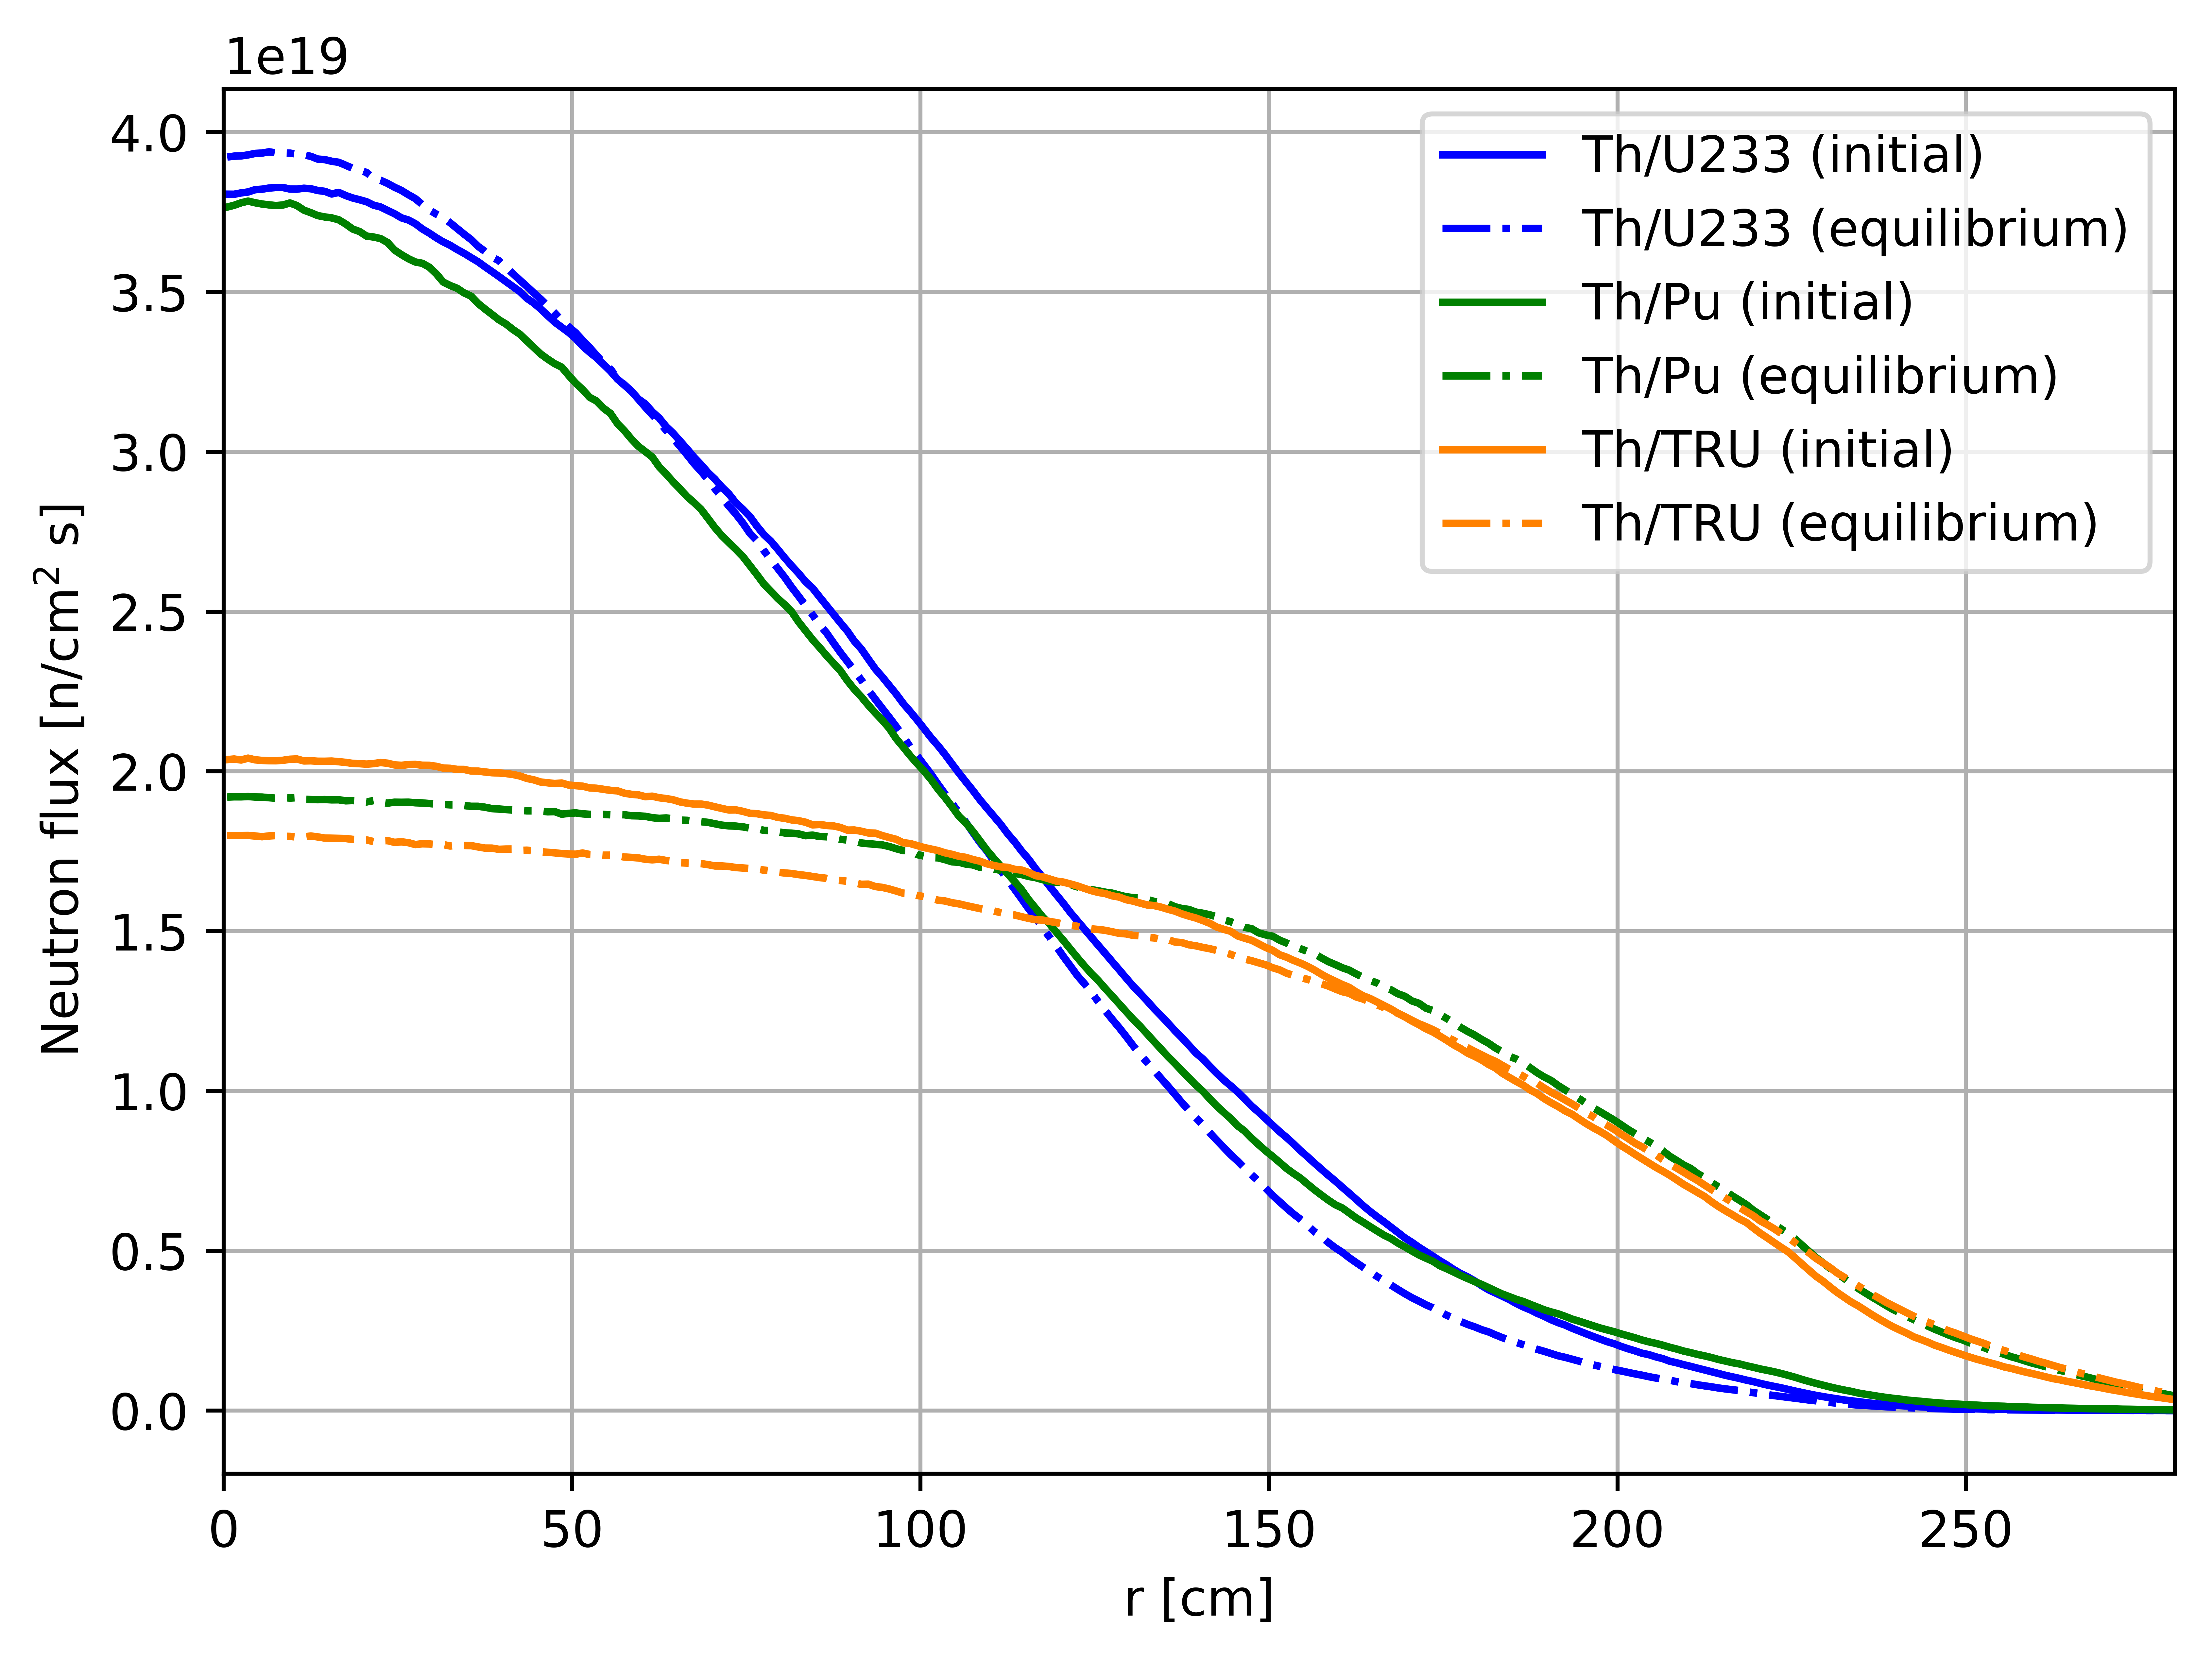
\includegraphics[width=\textwidth]{radial_fast_flux_init_vs_eq.png} 
	\caption{Radial fast neutron flux distribution for 3 different initial 
		fuel salt compositions at startup and equilibrium (the fast flux 
		confidence interval $\pm\sigma<2.5$\% for all cases).}
	\label{fig:fast_flux}
\end{figure}

Opposite behavior was observed for the Pu reactor-grade and TRU cases. For 
these cases, the thermal neutron flux is increasing during operation while 
fast neutron flux is decreasing. Fissile plutonium nuclides (generate 
relatively hard spectrum) from initial fuel salt composition is gradually 
substituted with the $^{233}$U (generates relatively soft spectrum), produced 
from the fertile $^{232}$Th. During reactor operation, the $^{233}$U becomes 
primary fissile isotope, which leads to the neutron spectrum softening of the 
reactor. 
\begin{figure}[htp!] % replace 't' with 'b' to force it to \centering
	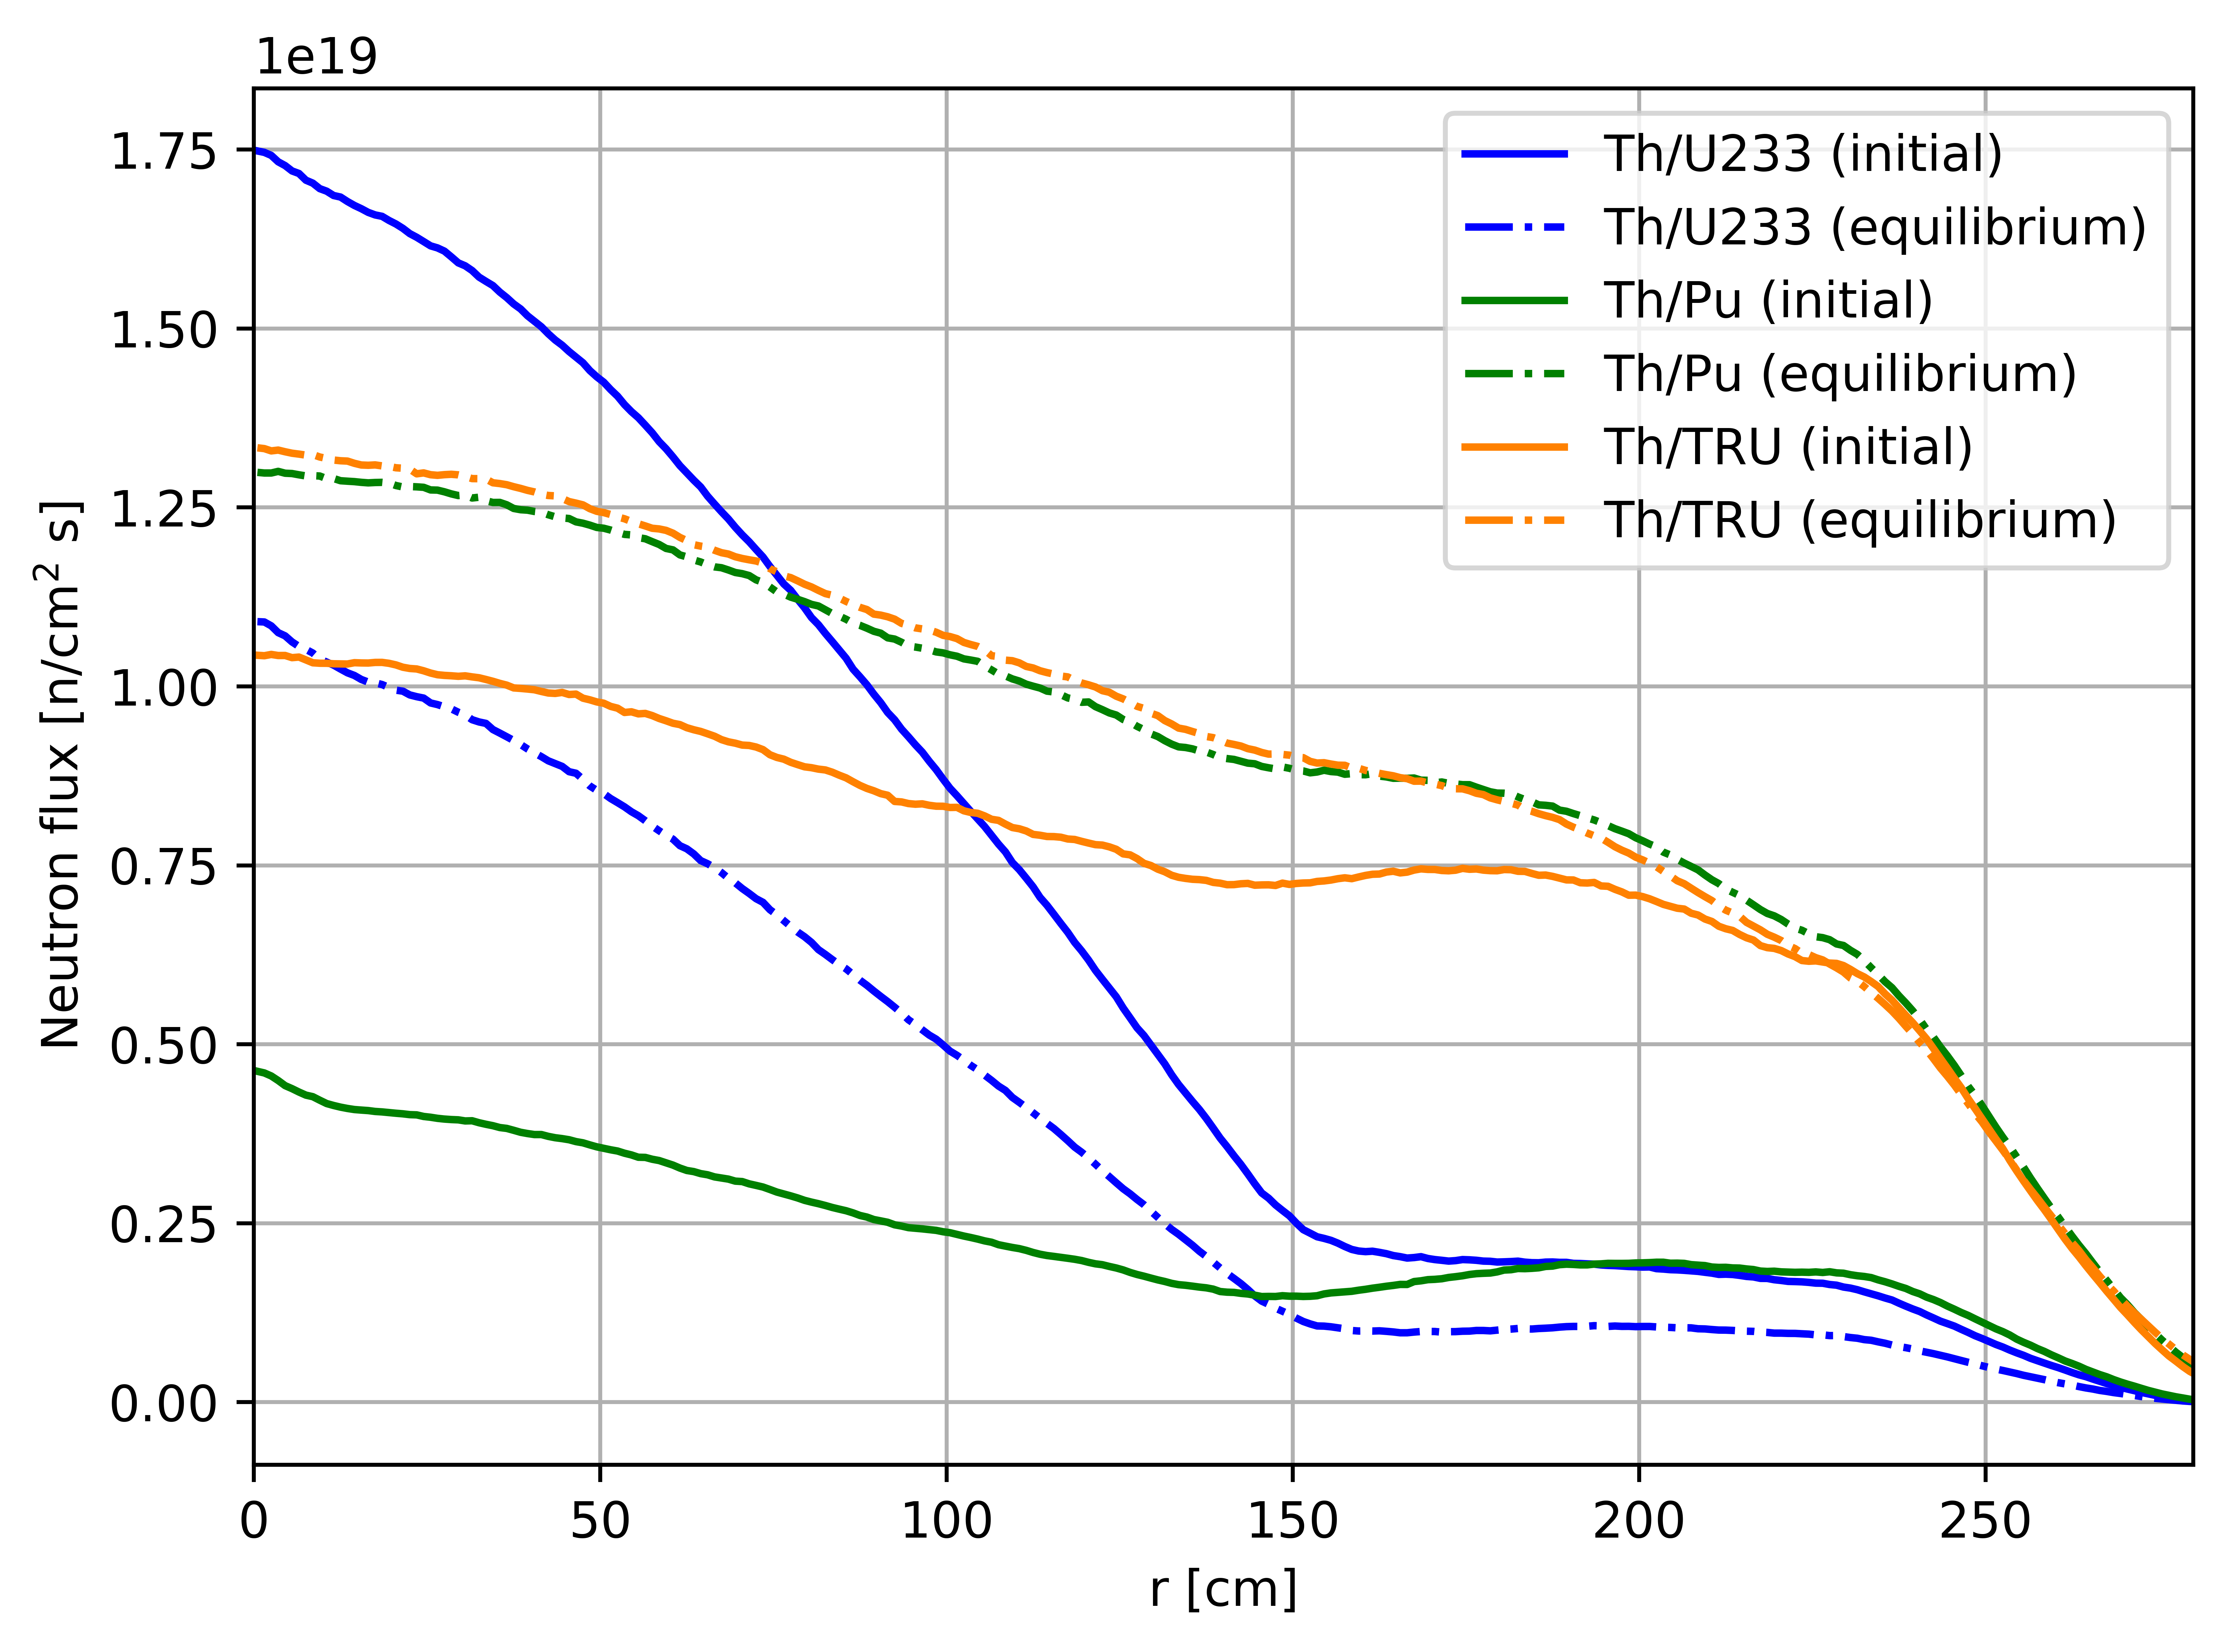
\includegraphics[width=\textwidth]{radial_thermal_flux_init_vs_eq.png} 
	\caption{Radial thermal neutron flux distribution for 3 different initial 
		fuel salt compositions at startup and equilibrium (the thermal flux 
		confidence interval $\pm\sigma<1.6$\% for all cases).}
	\label{fig:thermal_flux}
\end{figure}

Notably, more changes in thermal neutron flux shape and magnitude for  
$^{233}$U case were observed in the inner core zone ($R\lesssim150$) than 
in the outer core zone. In contrast, for Pu reactor-grade and TRU cases, 
significant changes were observed for thermal neutron flux in the outer core 
zone and reflector. Additionally, Figure~\ref{fig:thermal_flux} shows 
relatively large changes in thermal flux leakage from the core for the Pu and 
TRU cases. Overall, the SD-TMSR core design was optimized for $^{233}$U 
fissile isotope \cite{li_optimization_2018}; thus, the core geometry (e.g., 
fuel channels lattice pitch) must be re-optimized for another type of fuel to 
obtain better neutronics performance.

\subsection{Temperature coefficient of reactivity}
The temperature coefficient of reactivity quantifies reactivity changes due to 
temperature increase in the core and was calculated in this work as follows:
\begin{align}
\alpha &= \frac{k_{eff}(T_{i+1}) - k_{eff}(T_i)}{k_{eff}(T_{i+1}) 
	k_{eff}(T_{i}) (T_{i+1} - T_i)}
\intertext{where}
k_{eff} &= \mbox{effective multiplication factor} \nonumber \\
T_i &= \mbox{fuel salt temperature in (900 K, 1000 K).} \nonumber
\end{align}

Table~\ref{tab:tcoe} summarizes temperature coefficients calculated for three 
different initial fissile loads at the startup and at the equilibrium. By 
propagating the $k_{eff}$ statistical error provided by SERPENT-2, 
uncertainty for each temperature coefficient was calculated using formula:
\begin{align}
\delta\alpha &= \abs{\frac{1}{T_{i+1} - T_i}} \sqrt{\frac{\delta 
		k_{eff}^2(T_{i+1})}{k_{eff}^4(T_{i+1})}  
	+ \frac{\delta k_{eff}^2(T_i)}{k_{eff}^4(T_i)}}
\intertext{where}
\delta k_{eff} &= \mbox{statistical error for $k_{eff}$ from SERPENT-2 
output.} 
\nonumber
\end{align}
Notably, other sources of uncertainty are neglected, such as cross-section 
measurement error and approximations inherent in the density dependence on 
temperature. 

When the fuel salt temperature increases, the density of the salt decreases, 
but at the same time, the total volume of fuel salt in the 
core remains constant because it
is bounded by the vessel. When the graphite 
temperature increases, the density of
graphite decreases, creating additional 
space for the salt. The cross-section temperatures for the fuel and moderator 
were changed from 900 to 1000 K to determine the temperature coefficients. 
This work considered five different cases:
\begin{enumerate}
	\item Fuel salt temperature (Doppler Effect) rising from 900 to 1000 K 
	(first row  in Table ~\ref{tab:tcoe}).
	\item Fuel salt density decreasing from 3.3 to 3.233 g/cm$^3$ 
	(density change caused by temperature increase from	900 to 1000 K).
	\item Total fuel salt temperature (Doppler+density) rising from 900 to 
	1000 K.	
	\item Graphite temperature (Doppler Effect) rising from 900 to 1000 K.
	\item Whole reactor temperature rising from 900 K to 1000 K.
\end{enumerate}

In the first case, the fuel temperature change only impacts cross-section 
temperature. In the second case, changes in the fuel temperature only impact 
density, and the third case takes into account both effects. The geometry for 
these three cases is unchanged because the fuel is a liquid. However, when 
the graphite blocks heat up, both the density and the geometry changing due 
to the thermal expansion of solid graphite. The graphite linear thermal 
expansion is not a dominating factor \cite{li_optimization_2018}, and herein 
we focus only on Doppler Effect for the moderator temperature coefficient.
%%%%%%%%%%%%%%%%%%%%%%%%%%%%%%%%%%%%%%%%
\begin{table} [b!]
	\caption{Temperature coefficients of reactivity for 3 different initial 
		fuel salt compositions at startup and equilibrium. Confidence interval 
		$\pm\sigma$ for all coefficients is between $0.11$ and $0.16$ pcm/K).}
	\begin{tabularx}{\textwidth}{ p{0.27\textwidth} | X X  X X  X X } \hline
		\multirow{3}{*}{\shortstack{Reactivity coefficient \\ (pcm/K)}} 
		& 
		\multicolumn{6}{c}{Startup fissile material} \\ \cline{2-7}
		\space  & \multicolumn{2}{c}{$^{233}U$} & \multicolumn{2}{c}{Pu} & 
		\multicolumn{2}{c}{TRU} \\ \cline{2-7}
		\space  & Initial & Equil. & Initial & Equil. & Initial & 
		Equil. \\ \hline
		Fuel salt temperature&$-4.96$&$-5.26$&$-4.99$&$-3.12$&$-3.23$&$-1.97$ 
		\\ 
		Fuel salt density&$+1.49$&$+2.34$&$+1.54$&$-1.58$&$-0.37$&$-1.62$ \\
		Total salt fuel&$-3.77$&$-2.83$&$-3.22$&$-4.23$&$-3.25$&$-3.69$ \\ 
		\hline
		Graphite temperature&$+1.45$&$+0.45$&$-2.68$&$-1.37$&$-1.44$&$-1.14$ 
		\\	\hline
		Total core&$-1.77$&$-2.59$&$-6.54$&$-5.06$&$-4.79$&$-4.76$ \\ \hline
	\end{tabularx}
	\label{tab:tcoe}
\end{table}
%%%%%%%%%%%%%%%%%%%%%%%%%%%%%%%%%%%%%%%%%%%%%%%%%%%%%%%%%%%%%%%%%%%%%%%%%%%%%%%%

The \gls{FTC} is negative for all considered fuel compositions due to thermal 
Doppler broadening of the resonance capture cross-sections in the thorium. For 
$^{233}$U case, the \gls{FTC} decreases in magnitude by $-25\%$ due to neutron 
spectrum hardening during the reactor operation. For Pu reactor-grade and TRU 
cases, the \gls{FTC} becomes more negative at the equilibrium, by $+31\%$ and 
$+14\%$, respectively. Spectrum softening for these fueling cases positively 
affects the \gls{FTC} magnitude, and this effect seems to be proportional to 
the spectrum shift.

The \gls{MTC} for the $^{233}$U case is positive and decreases during reactor 
operation because of spectrum hardening with fuel depletion. For other cases, 
the \gls{MTC} is negative and also decreasing in magnitude during the reactor 
operation. Finally, the total temperature coefficient of reactivity is 
strongly negative for all considered scenarios but decreases in magnitude 
during reactor operation due to spectral shift. Notably, the total temperature 
coefficient is the most negative for the Pu reactor-grade case at startup, 
which has the hardest neutron spectrum (Figure~\ref{fig:spectrumFLUX110vC}). 
These coefficients agree with earlier estimates for SD-TMSR 
\cite{li_optimization_2018, ashraf2019whole_core} and \gls{MSBR} 
\cite{rykhlevskii2019modeling,  
rykhlevskii_full-core_2017,robertson_conceptual_1971}.

Even after 30 years of operation, the total temperature coefficient of 
reactivity remains relatively large and negative (in the range between $-2.59$ 
and $-5.06$ pcm/K) comparing with the conventional \gls{PWR}, which has 
temperature coefficient of about $-1.71$ $pcm/^{\circ}F\approx -3.08$ $pcm/K$ 
\cite{forget_integral_2018}), and allows excellent reactor stability and 
control. The additional analysis must be performed taking graphite moderator 
density change and linear thermal expansion into account, but material 
properties for the SD-TMSR graphite are not available in published literature. 
Alternatively, relatively well-studied reactor graphite (e.g., AXQ graphite 
\cite{robertson_conceptual_1971}) can be considered as a candidate for the 
SD-TMSR concept.

\subsection{Six Factor analysis}
The effective multiplication factor can be expressed as follows:
\begin{align}
k_{eff} &= k_{inf} P_f  P_t = \eta f p \epsilon P_f P_t
\intertext{where}
\eta     &= \mbox{thermal fission factor} \nonumber \\
f        &= \mbox{thermal utilization factor} \nonumber \\
p        &= \mbox{resonance escape probability} \nonumber \\
\epsilon &= \mbox{fast fission factor} \nonumber \\
P_f      &= \mbox{fast non-leakage probability} \nonumber \\
P_t      &= \mbox{thermal non-leakage probability.} \nonumber
\end{align}

Table~\ref{tab:six_factor} summarizes the six factors for 3 different initial 
fuel salt compositions at startup and equilibrium. By using SERPENT-2 built-in 
online reprocessing capabilities, all six factors have been calculated at the 
beginning of the operation and after 30 years of operation. Neutron population 
and number of active/inactive cycles were selected to obtain $k_{eff}$ 
statistical uncertainty less than 12 pcm. The fast and thermal non-leakage 
probabilities  remain constant regardless of initial fissile material and 
neutron spectrum shift during operation. The thermal utilization factor (f) 
remains almost constant during operation for $^{233}$U and TRU cases but 
considerably declines for Pu case due to significant neutron spectrum 
softening.
%%%%%%%%%%%%%%%%%%%%%%%%%%%%%%%%%%%%%%%%
\begin{table} [ht!]
	\caption{Six factors for the SD-TMSR model for 3 different initial 
		fuel salt compositions at startup and equilibrium.}
	\begin{tabularx}{\textwidth}{ X | X X  X X  X X } \hline
		\multirow{3}{*}{Factor}  & \multicolumn{6}{c}{Startup fissile 
			material} \\ \cline{2-7}
		\space  & \multicolumn{2}{c}{$^{233}U$} & \multicolumn{2}{c}{Pu} & 
		\multicolumn{2}{c}{TRU} \\ \cline{2-7}
		\space  & Initial & Equil & Initial & Equil & Initial & Equil \\ \hline
		$\eta$  & 1.26 & 1.40 & 1.66 & 1.44 & 1.59 & 1.31 \\ 
		f       & 0.97 & 0.98 & 0.96 & 0.76 & 0.80 & 0.75 \\
		p       & 0.54 & 0.43 & 0.26 & 0.16 & 0.17 & 0.15 \\
		$\epsilon$ & 1.49 & 1.67 & 2.45 & 5.87 & 4.83 & 6.81 \\
		P$_f$   & 0.99 & 0.99 & 0.99 & 0.99& 0.99 & 0.99 \\
		P$_t$   & 1.00 & 1.00 & 1.00 & 1.00 & 1.00 & 1.00 \\ \hline
	\end{tabularx}
	\label{tab:six_factor}
\end{table}
%%%%%%%%%%%%%%%%%%%%%%%%%%%%%%%%%%%%%%%%%%%%%%%%%%%%%%%%%%%%%%%%%%%%%%%%%%%%%%%%

In contrast, the neutron reproduction factor ($\eta$), resonance escape 
probability ($p$), and fast fission factor ($\epsilon$) differ notably between 
initial and equilibrium state for all three initial fissile materials. The 
fast fission factor ($\epsilon$) is much larger at startup for Pu and TRU 
cases because these initial fissile materials provided a much harder neutron 
spectrum than $^{233}$U, and $\epsilon$ grows throughout the core's lifetime. 
Conversely, the resonance escape probability decreases during reactor 
operation. The thermal fission factor increases during reactor operation for 
the $^{233}$U as initial fuel due to the accumulation of fissile plutonium 
isotopes, which produce more neutrons per fission ($\nu$). The other two 
scenarios demonstrated opposite behavior: plutonium isotopes with large 
neutrons per fission production ($\nu$) are gradually substituted with the 
$^{233}$U, which has lower $\nu$ \cite{sjostrand_cross_1960}. This six 
factors' evolution agrees with previously determined evolution parameters for 
a similar single-fluid double-zone \gls{MSBR} \cite{ashraf2019whole_core, 
rykhlevskii2019modeling, park_whole_2015}.